\documentclass[a4paper]{article}
\usepackage[utf8]{inputenc}
\usepackage[margin=1in, footskip=0.25in]{geometry}

\usepackage{booktabs}
\usepackage{graphicx}
\graphicspath{../plots}

\usepackage[backend=bibtex, style=numeric, sorting=none]{biblatex}
\bibliography{references}

\usepackage[font=footnotesize,labelfont=bf]{caption}
\captionsetup{width=\columnwidth}
\usepackage{subcaption}

\usepackage{listings}
\usepackage{xcolor}
\definecolor{backcolour}{RGB}{239,235,230}
\definecolor{lightgray}{gray}{0.7}
\lstdefinestyle{matlabcode}{
	language		=Matlab,
	backgroundcolor	=\color{backcolour},
	basicstyle		=\ttfamily\footnotesize,
	commentstyle	=\color{lightgray},
	numbers			=left,                    
	numbersep		=5pt,
	tabsize			=4,
	showstringspaces=false,
	frame			=leftline
}
\lstset{style=matlabcode}

\usepackage{amsmath}

\begin{document}
	
	% ======================= start titlepage ==============================================
	
	\begin{titlepage}
		\begin{center}
			\Large Numerical Methods in Astrophysics \\
			\vspace{1cm}
			\huge{
				Project 3 \\
				\vspace{0.5cm}
				\textbf{Two Dimensional Random Walk,}\\
				\textbf{Circular Binary and} \\
				\textbf{Hypervelocity Stars} \\
				\vspace{1cm}
			}
			\Large \emph{Saksham Kaushal}
		\end{center}
	\end{titlepage}
	
	% =========================end titlepage ================================================
	
	\tableofcontents
	\newpage
	
	% ========================= Problem 1 ===================================================
	
	\section{Problem1 - Two Dimensional Random Walk} \label{Problem1}
	
		% ------------------------------- Introduction --------------------------------------
		
		\subsection{Introduction} \label{1:introduction}
		
		% -------------------------------- Methods ------------------------------------------
		
		\subsection{Methods} \label{1:methods}
		
		\lstinputlisting[caption=first code,label=code:1.1]{../problem1/prob1aa.m}
		\lstinputlisting[caption=second code,label=code:1.2]{../problem1/prob1ab.m}
		\lstinputlisting[caption=third code,label=code:1.3]{../problem1/prob1ac.m}
		\lstinputlisting[caption=fourth code,label=code:1.4,
						firstline=28,firstnumber=28,
						lastline=35]{../problem1/prob1ad.m}
		
		% -------------------------------- Results ------------------------------------------
		 
		
		\subsection{Results} \label{1:results}
		\begin{figure}
			\begin{subfigure} {.5\columnwidth}
				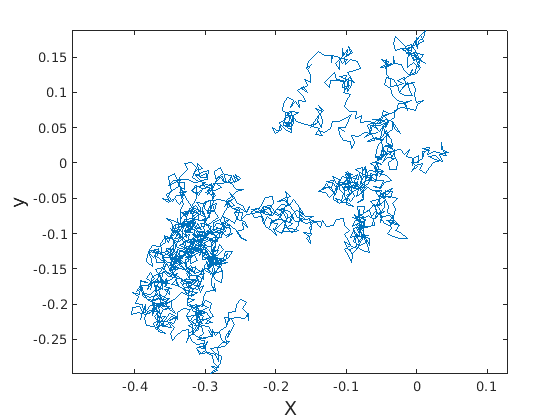
\includegraphics[width=\columnwidth]{../plots/1aa_randomwalk.png}
				\caption{1aa}
				\label{fig:1aa}
			\end{subfigure}%
			\hfill
			\begin{subfigure} {.5\columnwidth}
				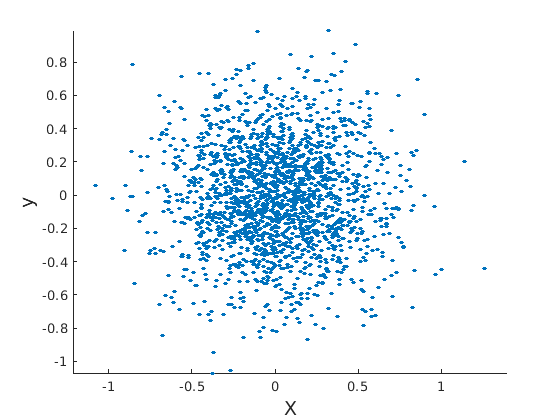
\includegraphics[width=\columnwidth]{../plots/1ab_randomwalk.png}
				\caption{1ab}
				\label{fig:1ab}
			\end{subfigure}
			
			\begin{subfigure} {.5\columnwidth}
				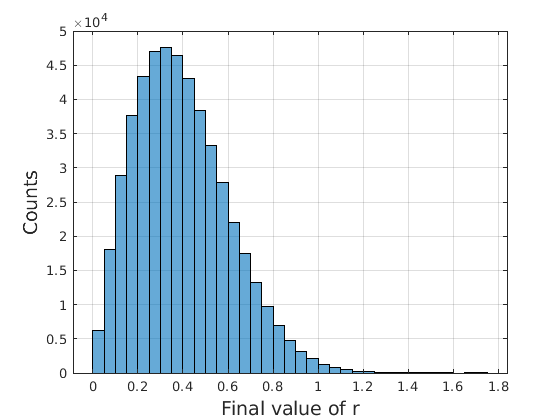
\includegraphics[width=\columnwidth]{../plots/1ac_hist_randomwalk.png}
				\caption{1ac}
				\label{fig:1ac}
			\end{subfigure}%
			\hfill
			\begin{subfigure} {.5\columnwidth}
				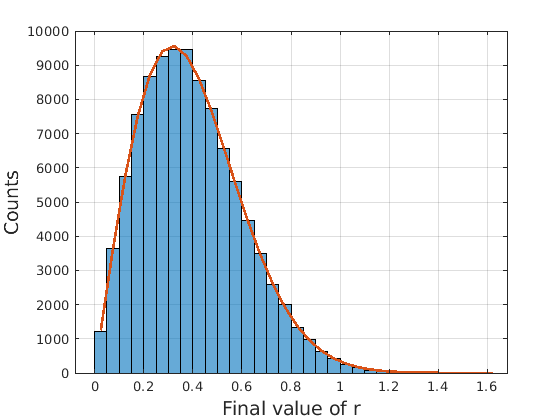
\includegraphics[width=\columnwidth]{../plots/1ad_hist_randomwalk.png}
				\caption{1ad}
				\label{fig:1ad}
			\end{subfigure}
			\caption{Problem 1.1}
			\label{fig:1}
		\end{figure}
		
		
		% -------------------------------- Discussions --------------------------------------
		
		\subsection{Discussions} \label{1:discussions}
	
	% ========================= Problem 1 ===================================================

	\section{Problem2 - Circular Binary} \label{Problem2}
	
		% ------------------------------- Introduction --------------------------------------

		\subsection{Introduction} \label{2:introduction}

		% -------------------------------- Methods ------------------------------------------

		\subsection{Methods} \label{2:methods}
		
		\lstinputlisting[caption=first code, label=code:2.1,
						firstline=7,firstnumber=9,
						lastline=19]{../problem2/binary.m}
		\lstinputlisting[caption=second code, label=code2.2,
						firstline=4]{../problem2/energyplot.m}

		% -------------------------------- Results ------------------------------------------

		\subsection{Results} \label{2:results}
		
		\begin{figure}
			\begin{subfigure} {.5\columnwidth}
				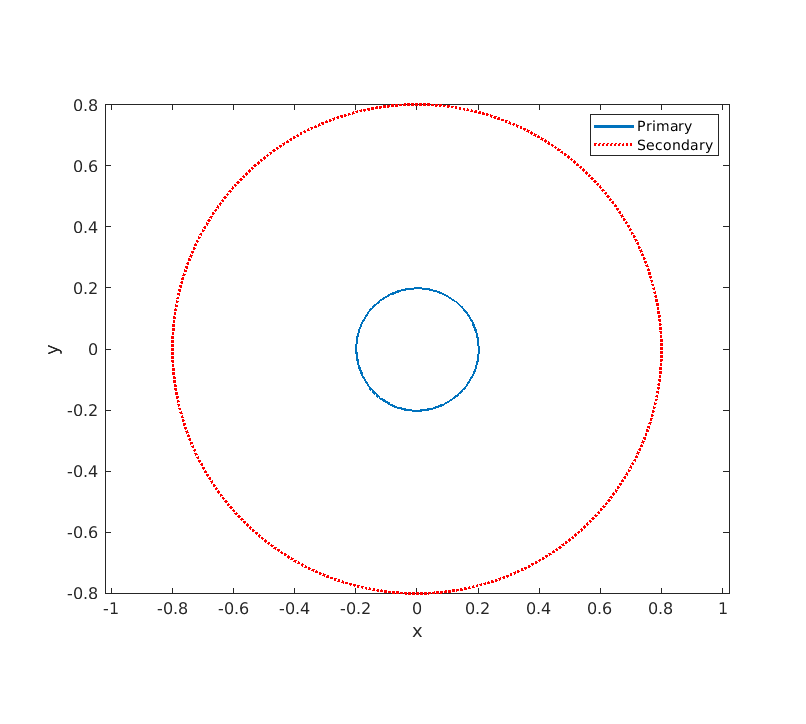
\includegraphics[width=\columnwidth]{../plots/2c_orbits.png}
				\caption{2c}
				\label{fig:2c}
			\end{subfigure}
			\hfill
			\begin{subfigure} {.5\columnwidth}
				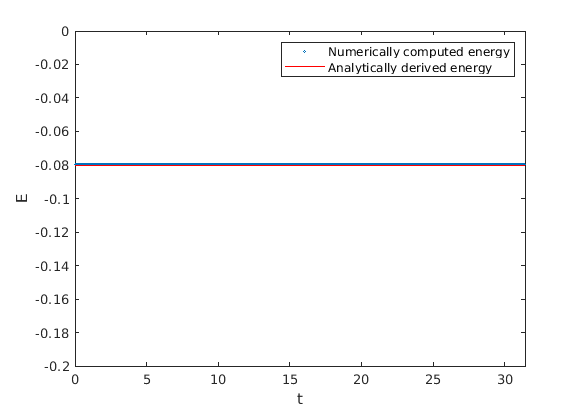
\includegraphics[width=\columnwidth]{../plots/2d_energies.png}
				\caption{2d}
				\label{fig:2d}
			\end{subfigure}
			\caption{Problem 2}
			\label{fig:2}
		\end{figure}

		% -------------------------------- Discussions --------------------------------------

		\subsection{Discussions} \label{2:discussions}


	% ========================= Problem 1 ===================================================

	\section{Problem3 - Hypervelocity Stars} \label{Problem3}
	
		% ------------------------------- Introduction --------------------------------------

		\subsection{Introduction} \label{3:introduction}

		% -------------------------------- Methods ------------------------------------------

		\subsection{Methods} \label{3:methods}
		
		\lstinputlisting[caption=code 1, label=code:3.initialc,
						firstline=5]{../problem3d/initialc.m}
		\lstinputlisting[caption=code 2, label=code:3.f]{../problem3d/f.m}

		% -------------------------------- Results ------------------------------------------

		\subsection{Results} \label{3:results}
		
		\begin{figure}
			\begin{subfigure} {.5\columnwidth}
				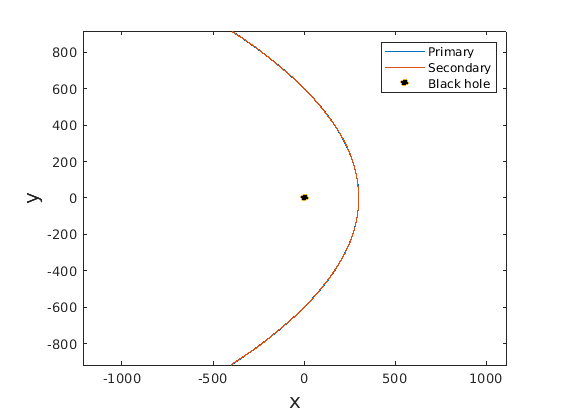
\includegraphics[width=\columnwidth]{../plots/3a_orbits_equalaxes.png}
				\caption{3a}
				\label{fig:3a}
			\end{subfigure}
			\hfill
			\begin{subfigure} {.5\columnwidth}
				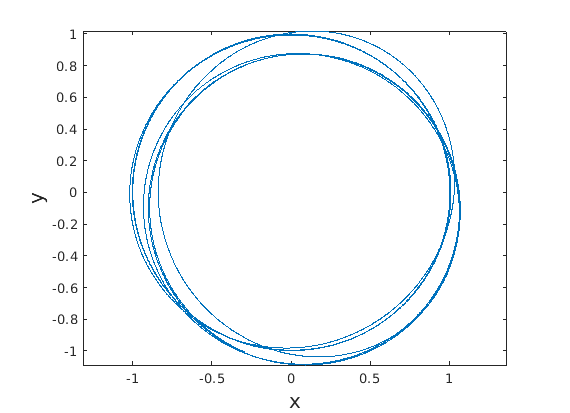
\includegraphics[width=\columnwidth]{../plots/3b_secondaryorbit.png}
				\caption{3b}
				\label{fig:3b}
			\end{subfigure}\\
			
			\begin{subfigure} {\columnwidth}
				\centering
				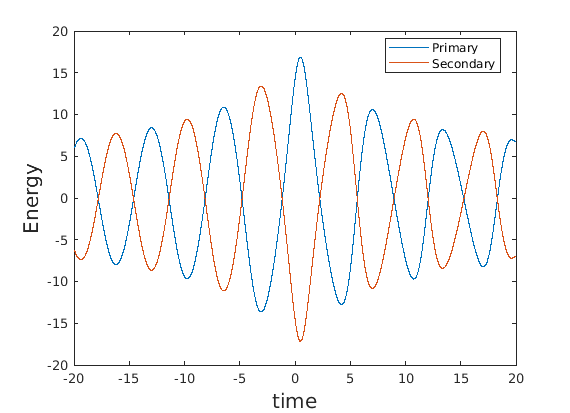
\includegraphics[width=.5\columnwidth]{../plots/3c_energy.png}
				\caption{3c}
				\label{fig:3c}
			\end{subfigure}
			\caption{Problem 3 - fig 1}
			\label{fig:3.1}
		\end{figure}
	
		\begin{figure}
			\begin{subfigure} {.5\columnwidth}
				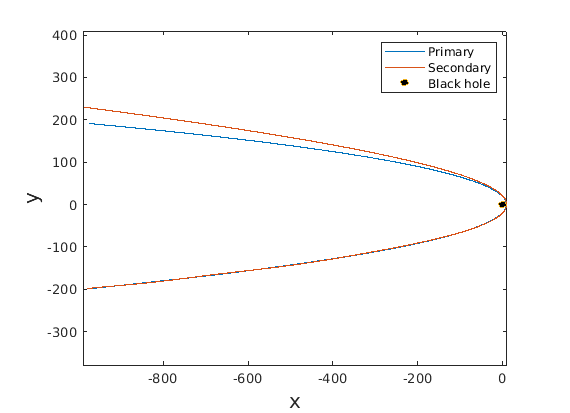
\includegraphics[width=\columnwidth]{../plots/3d_orbitsdisruption_equalaxes.png}
				\caption{3da}
				\label{fig:3da}
			\end{subfigure}
			\hfill
			\begin{subfigure} {.5\columnwidth}
				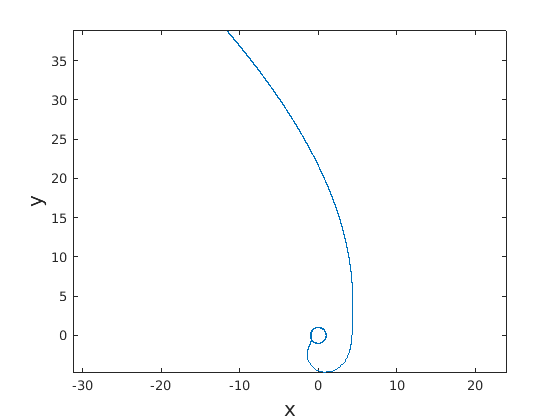
\includegraphics[width=\columnwidth]{../plots/3d_secondaryorbitdisruption_equalaxes.png}
				\caption{3db}
				\label{fig:3db}
			\end{subfigure}\\
			
			\begin{subfigure} {\columnwidth}
				\centering
				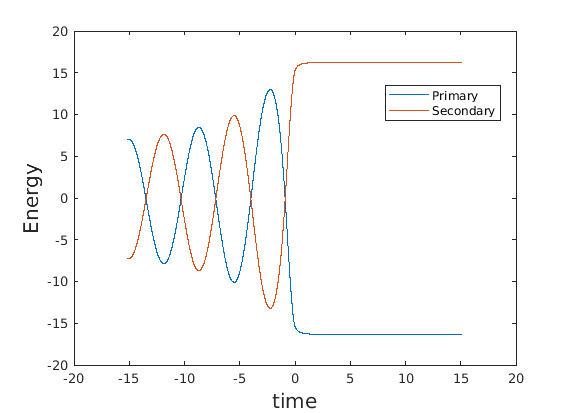
\includegraphics[width=.5\columnwidth]{../plots/3d_energy.png}
				\caption{3dc}
				\label{fig:3dc}
			\end{subfigure}
			\caption{Problem 3 - fig 2}
			\label{fig:3.2}
		\end{figure}
	
		\begin{table}
			\centering
			\begin{tabular} {l l r r}
				\toprule
				\textbf{Quantity} & \textbf{Variable} & \textbf{D=3} & \textbf{D=0.1}\\
				\midrule
				\(t^{}_{0}\) & \texttt{t} & -19.9555 & -15.1290 \\
				\(x^{}_{p}\) & \texttt{x(1)}& -400.0000 & -980.0000 \\
				\(y^{}_{p}\) & \texttt{x(2)} & -917.3151 & -199.7975 \\
				\(v^{}_{px}\) & \texttt{x(3)} & 37.6166 & 44.6972 \\
				\(v^{}_{py}\) & \texttt{x(4)} & 24.4949 & 4.4721 \\
				\(x^{}_{s}\) & \texttt{x(5)} & -400.0000 & -980.0000 \\
				\(y^{}_{s}\) & \texttt{x(6)} & -916.3151 & -198.7975 \\
				\(v^{}_{sx}\) & \texttt{x(7)} & 36.6166 & 43.6972 \\
				\(v^{}_{sy}\) & \texttt{x(8)} & 24.4949 & 4.4721 \\
				\bottomrule
			\end{tabular}
			\caption{Table of variable values for two values of D}
			\label{table:dvalues}
		\end{table}

		% -------------------------------- Discussions --------------------------------------

		\subsection{Discussions} \label{3:discussions}


\end{document}